\documentclass[
    11pt,
    %draft
]{beamer}
 
\usetheme{Antibes} % or Malmoe -> more somber

%% - - - - - - - - - - - - - - - - - - - - - - - - - - - - - - - - - - - - - %%
%%                               Load Packages                               %%
%% - - - - - - - - - - - - - - - - - - - - - - - - - - - - - - - - - - - - - %%

\usepackage[utf8]{inputenc} %% use UTF-8, maybe not needed since 2018
\usepackage[italian,main=english]{babel} %% language

\usepackage{csquotes} %% correct language also for citations

\usepackage[
  backend=biber,
  style=numeric,
  sorting=ynt
]{biblatex} %% for citations
\addbibresource{document.bib}

\usepackage{import} %% specify path for import

%% math packages
\usepackage{graphicx} %% for pictures
\usepackage{float}
\usepackage{amssymb} %% math symbols
\usepackage{amsmath} %% math matrix etc
\usepackage{minted} %% code block
\usepackage{tabularray} %% better tables
\usepackage{booktabs} %% rules for tables
\usepackage{mathrsfs}
\usepackage{mathtools}
\usepackage{algorithm} %% for algorithms
\usepackage{algpseudocode} %% loads algorithmicx
\usepackage{amsthm}
\usepackage{thmtools} %% theorems

%% plot packages
\usepackage{pgfplots} %% plots used with \begin{tikzpicture}
\usepackage{tikz} %% for pictures
\usetikzlibrary{trees}
\pgfplotsset{width=10cm,compat=newest}

%% design packages
\usepackage{enumitem} %% for lists and enumerating
\usepackage{color}
\usepackage{xcolor,colortbl} % xcolor for defining colors, colortbl for table colors
\usepackage{makecell} %% for multiple lines in cell of table
\usepackage{cancel}
\usepackage{pgfornament} %% ornaments



%% - - - - - - - - - - - - - - - - - - - - - - - - - - - - - - - - - - - - - %%
%%                       Configuration of the packages                       %%
%% - - - - - - - - - - - - - - - - - - - - - - - - - - - - - - - - - - - - - %%

\linespread{1}
\raggedbottom %% spaces if page is empty % chktex 1

%% set max table of contents recursion to subsection (3->subsubsecition)
\setcounter{tocdepth}{3}
\setcounter{secnumdepth}{3}

%% use bar instead of arrow for vectors
\renewcommand{\vec}[1]{\bar{#1}}
%% easy norm
\newcommand{\norm}[1]{\left\lvert#1\right\rvert}

% argmin and argmax
\DeclareMathOperator*{\argmax}{argmax}
\DeclareMathOperator*{\argmin}{argmin}

%% itemize use less vertical space (use olditemize for default behaviour)
\let\olditemize=\itemize%% old itemize
\let\endolditemize=\enditemize%% old end itemize
\renewenvironment{itemize}{\olditemize\itemsep-0.2em}{\endolditemize}

%% items in itemize emph+box
%% usage: \ieb{Class:} for simple item
%%        \ieb[4cm]{Class:} for specific size of box
\newcommand{\ieb}[2][2cm]{
        \makebox[#1][l]{\emph{#2}}
} %% TODO: replace with description environment (? maybe)

% section not in table of contents
\newcommand{\hiddensection}[1]{
  \stepcounter{section}
  \section*{{#1}}
}

\newcommand{\hiddensubsection}[1]{
  \stepcounter{subsection}
  \subsection*{{#1}}
}

% less vertical space around align & align*
\newcommand{\zerodisplayskips}{
  \setlength{\abovedisplayskip}{0pt}
  \setlength{\belowdisplayskip}{0pt}
  \setlength{\abovedisplayshortskip}{0pt}
  \setlength{\belowdisplayshortskip}{0pt}
}

% make dotfill use all the space available
\renewcommand{\dotfill}{
  \leavevmode\cleaders\hbox to 1.00em{\hss .\hss }\hfill\kern0pt } % chktex 1 chktex 26

\setlength{\fboxsep}{-\fboxrule} % for debugging


%% PACKAGE algorithm
\floatname{algorithm}{Algorithm}


%% PACKAGE tabularray
\UseTblrLibrary{amsmath}


%% PACKAGE color
\definecolor{red}{rgb}{1, 0.1, 0.1}
\definecolor{lightgreen}{rgb}{0.55, 0.87, 0.47}
\definecolor{gray}{rgb}{0.3, 0.3, 0.3}
\newcommand{\lgt}{\cellcolor{lightgreen}} %% light green in tables
\newcommand{\gry}{\textcolor{gray}} %% gray text
\newcommand{\rd}{\textcolor{red}} %% red text

%% PACKAGE minipage
\newcommand{\thend}[1]{\begin{center}
  \begin{minipage}[c][1em][c]{#1}
    \dotfill{}
  \end{minipage}
\end{center}}


%% PACKAGE thmtools
\declaretheoremstyle[
 headfont=\normalfont\bfseries,
 notefont=\mdseries,
 bodyfont=\normalfont,
 qed=\qedsymbol % chktex 1
]{steo}
\declaretheorem[numbered=no, style=steo]{mtheo}

\declaretheoremstyle[
  headfont=\normalfont\bfseries,
  notefont=\mdseries,
  bodyfont=\normalfont,
]{sdef}
\declaretheorem[numbered=no, style=sdef]{mdef}

\declaretheoremstyle[
  spaceabove=-6pt,
  spacebelow=6pt,
  headfont=\normalfont\bfseries,
  bodyfont=\normalfont,
  postheadspace=1em,
  qed=$\blacksquare$,
  headpunct={:}
]{sprf}
\declaretheorem[name={Proof}, style=sprf, numbered=no]{mproof}

%% ......................................................................... %%
%% local changes
% \setcounter{secnumdepth}{0}


%% - - - - - - - - - - - - - - - - - - - - - - - - - - - - - - - - - - - - - %%

\title{SEMINARIO}
\author{Elvis Rossi}
\institute[DEPARTMENT OF COMPUTER SCIENCE]{Department of Computer Science\\
  \medskip
  Master Degree in Computer Science
}
\date{\today}
\logo{\includegraphics[width=1cm]{figures/cherubino.eps}}

%% - - - - - - - - - - - - - - - - - - - - - - - - - - - - - - - - - - - - - %%

\begin{document}

\begin{frame}
  \titlepage % chktex 1
\end{frame}

\section*{Table of Contents}
\begin{frame}[allowframebreaks]
  \frametitle{Table of Contents}
  \tableofcontents
\end{frame}

\begin{section}{Introduction}

  % §§§§§§§§§§§§§§§§§§§§§§§§§§§§§§§§§§§§§§§§§§§§§§§§§§§§§§§§§§§§§§§§§§§§§§§§§§§§

  \begin{frame}\frametitle{Reaction Systems}
    \begin{tblr}{colspec={X[5,b]X[4,h]}, measure = vbox}
      {\begin{minipage}{\dimexpr\linewidth-\tabcolsep}\raggedright%
          RS is a qualitative model:
          \begin{itemize}
          \item[-] no permanency,
          \item[-] no counting.
          \end{itemize}

          \vspace{1em}

          Key concepts: \textit{Facilitation} and \textit{Inhibition}

          \vspace{1em}

          A reaction \((R, I, P)\) is composed by reactants, inhibitors and products.

          Reaction System: \(\mathcal{A} = (S, A)\)

          \vspace{1em}

          Behavior is not monotone.
        \end{minipage}} & {\captionsetup[figure]{font=tiny}\begin{figure}
          \includegraphics[clip, trim=20mm 110mm 85mm 40mm, width=0.8\linewidth, ]{figures/Molecular_Biology.pdf}
          \caption{Principle of Positive and Negative Regulation}
        \end{figure}} \\
    \end{tblr}

    % Reaction System (RS) is a successful computational framework inspired by biological systems.
    % S is called the background set of A and its elements are called entities
    % A is a set of reactions
  \end{frame}

  % §§§§§§§§§§§§§§§§§§§§§§§§§§§§§§§§§§§§§§§§§§§§§§§§§§§§§§§§§§§§§§§§§§§§§§§§§§§§

  \begin{frame}
    \begin{itemize}
    \item[-] Modeling and \textit{in silico} experiments,
    \item[-] Visualizing of LTS % labelled transition systems
    \item[-] Verifying properties: reachability, model checking, equivalence.
    \item[-] Analysis: causality, slicing, attractors, profiling.
    \item[-] Transformations: positive form, minimization.
    \end{itemize}
  \end{frame}
  
  % §§§§§§§§§§§§§§§§§§§§§§§§§§§§§§§§§§§§§§§§§§§§§§§§§§§§§§§§§§§§§§§§§§§§§§§§§§§§

  \begin{frame}\frametitle{Contribution}
    The main contribution is a rewrite of previous Prolog code in Rust.

    \vspace{1em}

    \begin{itemize}
    \item[-] ReactionSystems: contains the basic structures, parsers and a CLI.%
    \item[-] ReactionSystemsGUI:\ implements a native and web application with a custom visual language to interact with RS.%
    \end{itemize}
  \end{frame}

  % §§§§§§§§§§§§§§§§§§§§§§§§§§§§§§§§§§§§§§§§§§§§§§§§§§§§§§§§§§§§§§§§§§§§§§§§§§§§

  \begin{frame}\frametitle{Example}
    \begin{figure}[h]
      \includegraphics[width=0.9\textwidth]{figures/instructions_medical.png}
    \end{figure}
    \begin{figure}[h]
      \includegraphics[width=0.9\textwidth]{figures/output_medical.png}
    \end{figure}
  \end{frame}
  % §§§§§§§§§§§§§§§§§§§§§§§§§§§§§§§§§§§§§§§§§§§§§§§§§§§§§§§§§§§§§§§§§§§§§§§§§§§§
\end{section}

% ==============================================================================

\begin{section}{Design}
  % §§§§§§§§§§§§§§§§§§§§§§§§§§§§§§§§§§§§§§§§§§§§§§§§§§§§§§§§§§§§§§§§§§§§§§§§§§§§
  \begin{frame}\frametitle{Structure}
    The libraries are more than 30k lines of code, organized in workspaces that allow easy development; the visual language has 29 types and more than 70 node operations.

    \begin{figure}[!h]
      \centering
      \scalebox{0.55}{
        \begin{tikzpicture}[
          place/.style={rectangle,draw=blue!50,fill=blue!20,thick},
          >=Stealth, thick, every node/.style={font=\sffamily}]

          \node[place] (analysis)          at (0,0.1)  {analysis};
          \node[place] (grammar)           at (3,-2)  {grammar};
          \node[place] (grammarseparated) at (-3,-2) {grammar\_separated};
          \node[place] (execution)         at (0,-1)  {execution};
          \node[place] (bisimilarity)      at (-3,-1) {bisimilarity};
          \node[place] (assert)            at (0,-2)  {assert};
          \node[place] (rsprocess)         at (0,-3)  {rsprocess};

          \draw[->]              (rsprocess) -- (assert);
          \draw[->]              (rsprocess) -- (grammarseparated);
          \draw[->,bend right=35](rsprocess) to[bend right=55] (execution);
          \draw[->]              (rsprocess) -- (grammar);
          \draw[->,bend right=32](rsprocess) to[bend right=57] (analysis);

          \draw[->]              (assert) -- (execution);
          \draw[->]              (assert) -- (grammarseparated);
          \draw[->]              (assert) -- (grammar);

          \draw[->]              (execution) -- (analysis);
          \draw[->]              (execution) -- (grammarseparated);
          \draw[->]              (execution) -- (grammar);

          \draw[->]              (bisimilarity) -- (execution);

          \draw[->]              (grammar) to[bend right=10] (analysis);
        \end{tikzpicture}
      }
      \scalebox{0.55}{
        \begin{tikzpicture}[scale=0.8, every node/.style={scale=0.8},
          place/.style={rectangle,draw=blue!50,fill=blue!20,thick},
          >=Stealth, thick, every node/.style={font=\sffamily}]

          \node[place] (set)     at (0,3)    {Set};
          \node[place] (reaction)at (4,3)    {Reaction};
          \node[place] (choices) at (8,3)    {Choices};
          \node[place] (label)   at (-2,1.5) {Label};
          \node[place] (env)     at (2,1.5)  {Environment};
          \node[place] (process) at (6,1.5)  {Process};
          \node[place] (system)  at (4,0)    {System};
          \node[place] (graph)   at (0,0)    {Graph};

          % Set
          \draw[->]              (set) -- (reaction);
          \draw[->,bend left=18] (set) to (choices);
          \draw[->,bend right=25](set) to (label);
          \draw[->]              (set) -- (graph);
          \draw[->,bend right=35,looseness=1.1] (set) to (system);
          \draw[->,bend right=12](set) to (env);

          % Label -> Graph
          \draw[->] (label) -- (graph);

          % Reaction
          \draw[->,bend left=12]  (reaction) to (process);
          \draw[->,bend right=12] (reaction) to (env);
          \draw[->,bend left=16]  (reaction) to (system);

          % Process
          \draw[->]               (process) -- (env);
          \draw[->]               (process) -- (system);
          \draw[->,bend right=18] (process) to (choices);

          \draw[->] (choices) to [bend left=2] (env);
          \draw[->] (choices.south) to [bend left=25] (system.east);
          \draw[->]               (env) -- (system);
          \draw[<->,bend left=15] (system) to (graph);
        \end{tikzpicture}
      }
    \end{figure}

    Grammars have been specified and developed for the RS structures using \(\texttt{lalrpop}\).
  \end{frame}

  % §§§§§§§§§§§§§§§§§§§§§§§§§§§§§§§§§§§§§§§§§§§§§§§§§§§§§§§§§§§§§§§§§§§§§§§§§§§§
  \begin{frame}\frametitle{SOS rules}
    \begin{tblr}{colspec={Q[c,m]Q[l,m]}}
      {\begin{bnf}(relation-sym-map = % chktex 36
        {
          {::=} = {\ensuremath{\Coloneqq}},
          {->} = {},
          {:in:} = {\ensuremath{\subseteq}},
        },)
        $P$ : ::= % chktex 26
        | [$M$] : % chktex 26
        ;; % chktex 26
        $M$ : ::= % chktex 26
        | $(R, I, P)$ : % chktex 26
        | $D$ : % chktex 26
        | $K$ : % chktex 26
        | $M \vert M$ : % chktex 26
        ;; % chktex 26
        $K$ : ::= % chktex 26
        | \textbf{$0$} : % chktex 26
        | $X$ : % chktex 26
        | $C.K$ : % chktex 26
        | $K + K$ : % chktex 26
        | $\texttt{rec} X . K$ : % chktex 26
      \end{bnf}} & {Mutual Exclusion of 2 looping processes:\\
      \vspace{1em}
      {\tt Environment: [\\
      \quad k1 = (\{\}.k1 + \{act\_1\}.k1),\\
      \quad k2 = (\{\}.k2 + \{act\_2\}.k2)\\
      ]\\
      Initial Entities: \{out\_1, out\_2\}\\
      Context: [k1, k2]\\
      Reactions: (}\(\ldots\){\tt)}}\\ % chktex 9
    \end{tblr}
    % structured operational semantics
    % The behavior of a RS could be defined as a discrete time interactive
    % process: a finite context sequence describes the entities provided by the
    % environment at each step, the current state is determined by the union of
    % the entities coming from the environment with those produced from the
    % previous step and the state sequence is determined by applying all and
    % only the enabled reactions to the set of entities available in the current
    % state

    % (R, I, P) is a reaction, D is a set of entities (a reaction that is always
    % enabled), | (pipe) is the parallel composition

    % 0 is the nil context written as nill, X is a process variable, C is a set
    % of entities, + is non deterministic choice, rec is the recursive operator

    % operational semantics follow the definitions
  \end{frame}

  % §§§§§§§§§§§§§§§§§§§§§§§§§§§§§§§§§§§§§§§§§§§§§§§§§§§§§§§§§§§§§§§§§§§§§§§§§§§§

  \begin{frame}{Graphs}
    To explore the structure of RSs, methods are provided to create and manipulate graphs.

    \begin{tblr}{colspec={Q[l,b]Q[l,b]},width=\linewidth}
      {\includegraphics[scale=0.16]{figures/graph_instructions.png}} & {
                                                                       Domain specific languages have been\\developed for:
      \begin{itemize}
      \item[$-$] specifying labels of nodes \& edges,
      \item[$-$] specifying color of nodes \& edges,
      \item[$-$] grouping of nodes,
      \item[$-$] relabeling of edges.
      \end{itemize}} \\
    \end{tblr}
  \end{frame}

  % §§§§§§§§§§§§§§§§§§§§§§§§§§§§§§§§§§§§§§§§§§§§§§§§§§§§§§§§§§§§§§§§§§§§§§§§§§§§

  \begin{frame}
    \begin{figure}[h]
      \includegraphics[width=0.95\textwidth]{figures/lock_instructions.png}
    \end{figure}

    \begin{figure}[h]
      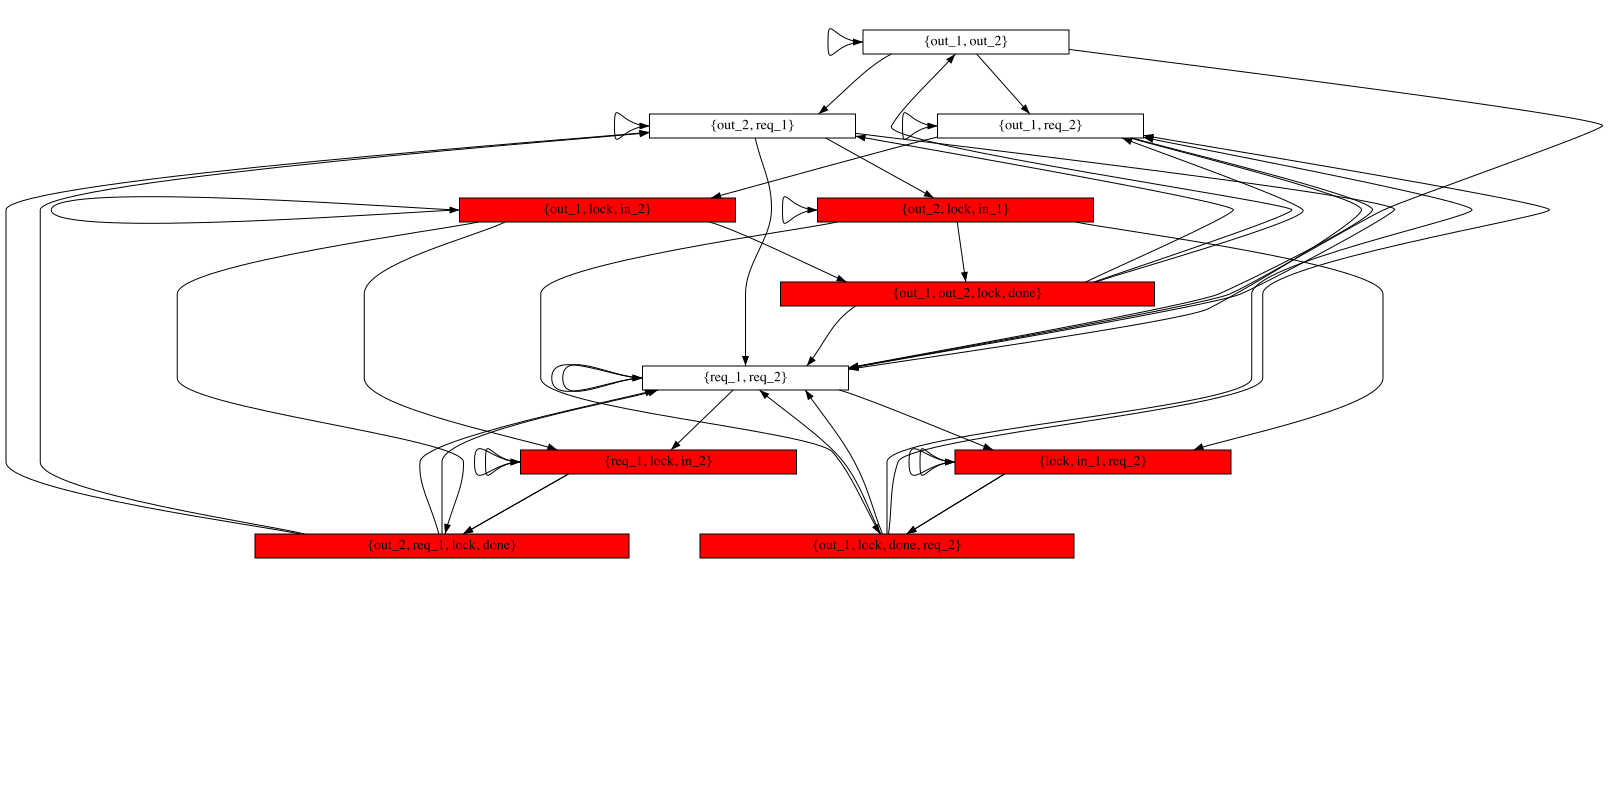
\includegraphics[scale=0.2]{figures/lock.pdf}
    \end{figure}
  \end{frame}

  % §§§§§§§§§§§§§§§§§§§§§§§§§§§§§§§§§§§§§§§§§§§§§§§§§§§§§§§§§§§§§§§§§§§§§§§§§§§§

  \begin{frame}\frametitle{Positive Reaction Systems}
    Instead of considering the absence of an element, consider the presence of a negative element:

    \vspace{0.5em}

    Reaction: \((R, P)\)

    \vspace{0.5em}

    An equivalent Positive RS can be built for each RS.%
    \begin{figure}[h]
      \includegraphics[width=0.9\textwidth]{figures/to_positive_reactions.png}
    \end{figure}

    % To convert a list of reactions we first create a reaction for each product
    % in each reaction, then all reactions that have the same product are
    % converted together into their positive versions: One reaction is simply
    % the positive reactants and the negative inhibitors that produce the
    % positive product. The others are related to the absence of the product and
    % are created from the prohibiting set, where for every reactants or
    % inhibitor that does not allow the reaction to be enabled a reaction is
    % created.

    % The resulting reactions are then minimized, in order to reduce the
    % complexity of the traces, even tho the behavior is the same.
  \end{frame}

  % §§§§§§§§§§§§§§§§§§§§§§§§§§§§§§§§§§§§§§§§§§§§§§§§§§§§§§§§§§§§§§§§§§§§§§§§§§§§

  \begin{frame}\frametitle{Slicing}
    Dynamic slicing is a technique that helps a user to debug a program by simplifying a partial execution trace.

    The goal is to highlight how a subset of the elements in a state were originated.

    \begin{minipage}{\textwidth}
      \centering
      \begin{minipage}[t][0.5\textheight][t]{0.75\textwidth}
        \begin{figure}
          \includegraphics[height=0.5\textheight]{figures/positive_slice.png}
        \end{figure}
      \end{minipage}%
      \begin{minipage}[t][0.5\textheight][t]{0.25\textwidth}
        \begin{figure}
          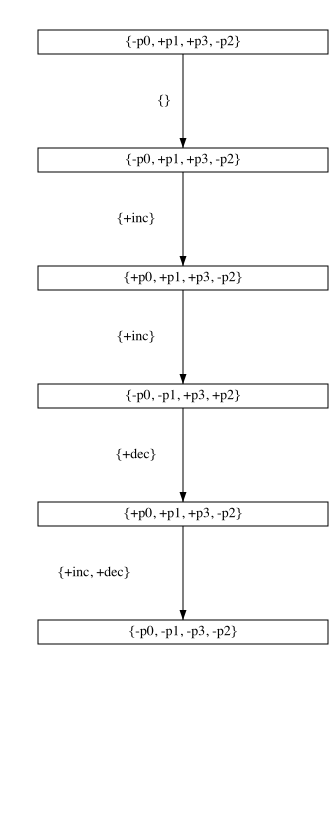
\includegraphics[scale=0.25]{figures/counting.pdf}
        \end{figure}
      \end{minipage}
    \end{minipage}
  \end{frame}

  % §§§§§§§§§§§§§§§§§§§§§§§§§§§§§§§§§§§§§§§§§§§§§§§§§§§§§§§§§§§§§§§§§§§§§§§§§§§§
  \begin{frame}\frametitle{Bisimulation}
    A common question given two RS processes is if they behave the same.
    Bisimulation is a binary relation between transition systems defined in therms of coinductive games, of fixed point theory and of logic.

    Two algorithms have been implemented: by Kanellakis and Smolka, and by Paige and Tarjan.

    \begin{figure}
      \includegraphics[scale=0.25]{figures/bisimilarity.png}
    \end{figure}
  \end{frame}

  % §§§§§§§§§§§§§§§§§§§§§§§§§§§§§§§§§§§§§§§§§§§§§§§§§§§§§§§§§§§§§§§§§§§§§§§§§§§§
  \begin{frame}\frametitle{Kanellakis and Smolka}
    The algorithm by Kanellakis and Smolka is based on the concept of splitter.

    \begin{tikzpicture}[baseline,
      place/.style={circle,draw=blue!50,fill=blue!20,thick},
      >=Stealth, thick, every node/.style={font=\sffamily}]

      \node[place] (s1) at (0,0) {\(s_1\)};
      \node[place] (s2) at (2,0) {\(s_2\)};
      \node[place] (s3) at (4,0) {\(s_3\)};
      \node[place] (s4) at (1,-2) {\(s_4\)};
      \node[place] (s5) at (3,-2) {\(s_5\)};

      \draw[->]    (s1) -- (s4);
      \draw[->]    (s2) -- (s5);

      \draw[->]    (s2) to[bend left=20] (s3);
      \draw[->]    (s3) to[bend left=20] (s2);

      \node[draw=black!80,fit=(s1) (s2) (s3),label=above right:$B_1$] {};
      \node[draw=black!80,fit=(s4) (s5),label=below right:$B_2$] {};
    \end{tikzpicture}%
    \hspace{0.3em}\(\to\)\hspace{0.3em}%
    \begin{tikzpicture}[baseline,
      place/.style={circle,draw=blue!50,fill=blue!20,thick},
      >=Stealth, thick, every node/.style={font=\sffamily}]

      \node[place] (s1) at (0,0) {\(s_1\)};
      \node[place] (s2) at (2,0) {\(s_2\)};
      \node[place] (s3) at (4,0) {\(s_3\)};
      \node[place] (s4) at (1,-2) {\(s_4\)};
      \node[place] (s5) at (3,-2) {\(s_5\)};

      \draw[->]    (s1) -- (s4);
      \draw[->]    (s2) -- (s5);

      \draw[->]    (s2) to[bend left=20] (s3);
      \draw[->]    (s3) to[bend left=20] (s2);

      \node[draw=blue!80,fit=(s1) (s2),label=above right:$B_1$] {};
      \node[draw=blue!80,fit=(s3),label=above:$B_3$] {};
      \node[draw=black!80,fit=(s4) (s5),label=below right:$B_2$] {};
    \end{tikzpicture}%
  \end{frame}

  % §§§§§§§§§§§§§§§§§§§§§§§§§§§§§§§§§§§§§§§§§§§§§§§§§§§§§§§§§§§§§§§§§§§§§§§§§§§§

  \begin{frame}\frametitle{Paige and Tarjan}
    The algorithm by Kanellakis and Smolka has time complexity \(O(n \cdot m)\).
    % where n is the number of states and m is the number of transitions
    By reducing to the coarsest stable partition problem, the complexity can be reduced to \(O(n \cdot \log(m))\), since three-way splitting can be performed in time proportional to the size of the smaller of the two blocks.
    % additional structures are needed for bookkeeping

    \vspace{1em}

    The algorithm is specified over systems with only one action, but other systems can be transformed into equivalent ones.


    \begin{tblr}{width=\linewidth, colspec={X[r]Q[c]X[l]}}
      \begin{tikzpicture}[auto,
        place/.style={rectangle,draw=blue!50,fill=blue!20,thick,inner sep=0pt,
          minimum size=6mm},
        pre/.style={<-,shorten <=1pt,>={Stealth[round]},semithick},
        post/.style={->,shorten >=1pt,>={Stealth[round]},semithick}
        ]
        \node[place] (P1)               {\(P_1\)};
        \node[place] (P2) [right=of P1] {\(P_2\)}
        edge [pre] node [auto, swap] {\(\alpha_1\)} (P1);
        \node[place] (P3) [below=of P2] {\(P_3\)}
        edge [pre] node [auto] {\(\alpha_2\)} (P1)
        edge [pre] node [auto, swap] {\(\alpha_2\)} (P2);
      \end{tikzpicture}
      & \(\raisebox{3.5em}{\to}\) &
        \scalebox{0.30}{
        \begin{tikzpicture}[auto,
          place/.style={rectangle,draw=blue!50,fill=blue!20,thick,inner sep=0pt,
            minimum size=6mm},
          new/.style={circle,draw=blue!30,fill=blue!10,thick,inner sep=0pt,
            minimum size=6mm},
          pre/.style={<-,shorten <=1pt,>={Stealth[round]},semithick},
          post/.style={->,shorten >=1pt,>={Stealth[round]},semithick}
          ]
          \node[place] (P1) {\(P_1\)};
          \node[new] (p1e1) [above=of P1] {}
          edge [pre] (P1);
          \node[new] (p1e2) [above=of p1e1] {}
          edge [pre] (p1e1);
          \node[new] (p1e3) [above=of p1e2] {}
          edge [pre] (p1e2);

          \node[new] (a1) [right=of P1] {}
          edge [pre] (P1);
          \node[new] (a1e1) [above=of a1] {}
          edge [pre] (a1);

          \node[place] (P2) [right=of a1] {\(P_2\)}
          edge [pre] (a1);
          \node[new] (p2e1) [above=of P2] {}
          edge [pre] (P2);
          \node[new] (p2e2) [above=of p2e1] {}
          edge [pre] (p2e1);
          \node[new] (p2e3) [above=of p2e2] {}
          edge [pre] (p2e2);

          \node[new] (a2) [below=of P2] {}
          edge [pre] (P2);
          \node[new] (a2e1) [right=of a2] {}
          edge [pre] (a2);
          \node[new] (a2e2) [right=of a2e1] {}
          edge [pre] (a2e1);

          \node[new] (a3) [below=of a1] {}
          edge [pre] (P1);
          \node[new] (a3e1) [below=of a3] {}
          edge [pre] (a3);
          \node[new] (a3e2) [below=of a3e1] {}
          edge [pre] (a3e1);

          \node[place] (P3) [below=of a2] {\(P_3\)}
          edge [pre] (a2)
          edge [pre] (a3);
          \node[new] (p3e1) [right=of P3] {}
          edge [pre] (P3);
          \node[new] (p3e2) [right=of p3e1] {}
          edge [pre] (p3e1);
          \node[new] (p3e3) [right=of p3e2] {}
          edge [pre] (p3e2);
        \end{tikzpicture}
        }
    \end{tblr}
    % The operation is log-space
  \end{frame}

  % §§§§§§§§§§§§§§§§§§§§§§§§§§§§§§§§§§§§§§§§§§§§§§§§§§§§§§§§§§§§§§§§§§§§§§§§§§§§

  \begin{frame}\frametitle{Testing}
    During the development to validate the program automated tests and manual integration have been used.

    \begin{figure}[h]
      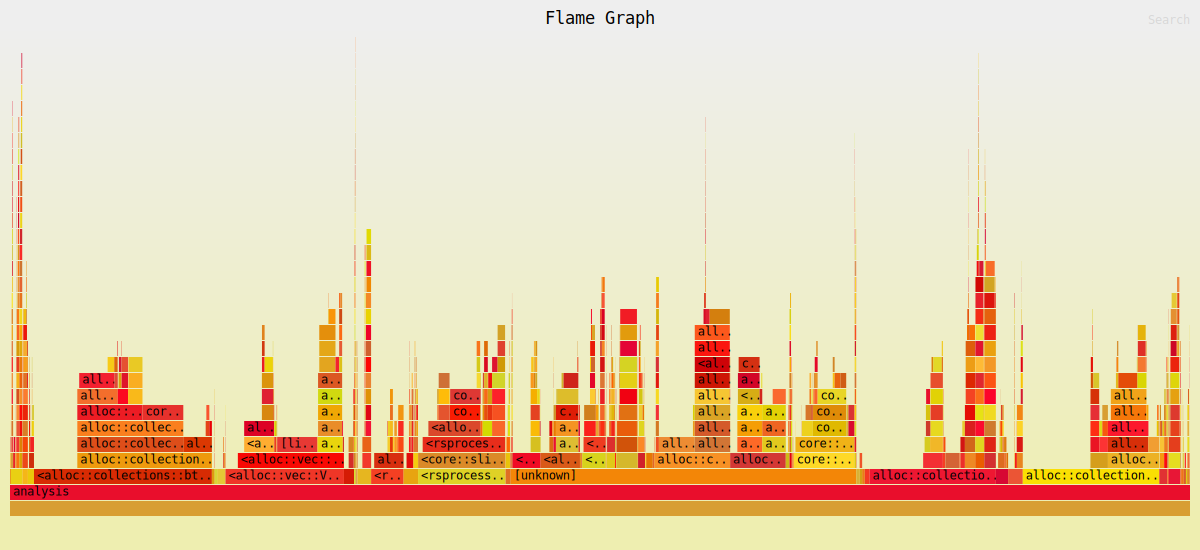
\includegraphics[scale=0.2]{figures/flamegraph_mex10.pdf}
      \caption{Profiling using \(\texttt{perf}\) and \(\texttt{flamegraph}\).}
    \end{figure}
    % 3k lines of tests
  \end{frame}

  % §§§§§§§§§§§§§§§§§§§§§§§§§§§§§§§§§§§§§§§§§§§§§§§§§§§§§§§§§§§§§§§§§§§§§§§§§§§§

\end{section}

% ==============================================================================

\begin{section}{Conclusion}
  
  % §§§§§§§§§§§§§§§§§§§§§§§§§§§§§§§§§§§§§§§§§§§§§§§§§§§§§§§§§§§§§§§§§§§§§§§§§§§§

  \begin{frame}\frametitle{Conclusion}
    Key contributions:
    \begin{itemize}
    \item[$\bullet$] New RS modeling platform that aids in analysis and design, implemented in 30k lines of Rust. Provides a CLI and a GUI.%
    \item[$\bullet$] Comprehensive Feature Set: simulation of RS, bisimulation of graphs, trace slicing, graph generation with Dot, GraphML and SVG outputs, loop analysis, automated conversion between RS types.
    \item[$\bullet$] Improved performance and usability compared to previous software written in Prolog and Python.
    \end{itemize}
  \end{frame}

  % §§§§§§§§§§§§§§§§§§§§§§§§§§§§§§§§§§§§§§§§§§§§§§§§§§§§§§§§§§§§§§§§§§§§§§§§§§§§

\end{section}

\begin{frame}

\end{frame}


\end{document}

%% - - - - - - - - - - - - - - - - - - - - - - - - - - - - - - - - - - - - - %%

%%% Local Variables:
%%% TeX-command-extra-options: "-shell-escape"
%%% End:
